\chapter{Generative models}
\section{Restricted Boltzmann Machines}
The Boltzmann Machines come under the category of Energy Based Models. The name energy based models is given because they make use of Boltzmann distribution also known as Gibbs distribution which is a part of statistical models that helps in determining the quantum state parameters like Entropy, Temperature etc.   These Botlzmann models are stochastic generative deep learning models that have only two nodes namely hidden and visible nodes. Like conventional neural network models, they explicitly do have output nodes with 0 or 1 states through which they learns the patterns. Each of the nodes of these models are linked to one another irrespective of they type (either input or hidden) and do they learn and share the information among these nodes. This makes them non-deterministic and since they self generate the subsequent data, they are known as deep generative models. A Restricted Boltzmann machine (RBM) is a generative two-layered neural network model with restrictions in its hidden and visible nodes. They have the capability to learn a probability distribution given a set of observations. In this exercise, we evaluate the performance of a RBM on MNIST digits dataset. We train the RBM with different parameters like number of iterations, number of components, gibbs sampling steps etc. The model is then evaluated on unseen images for each of the configuration. To first analyze the effect of training parameters like number of components, number of iterations etc. we keep the gibbs sampling steps to  constant value of 20, learning rate to 0.01, batch size to 10 and change the training parameters and the results are as given below.
\begin{figure}[ht]
	\begin{subfigure}[b]{0.33\textwidth}
		\centering
		\captionsetup{ width=0.8\linewidth, format = hang}
		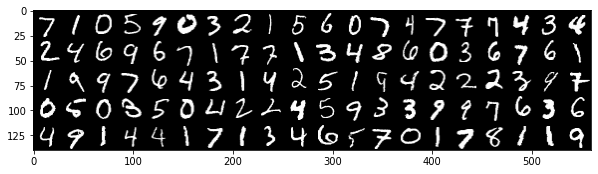
\includegraphics[height = 0.5\textwidth, width = 1\textwidth]{Exercise4/Report/test_image}
		\caption{Test Images from the MNIST data set}\label{fig:test}
	\end{subfigure}%
	\begin{subfigure}[b]{0.33\textwidth}
		\centering
		\captionsetup{width=0.8\linewidth, format = hang}
		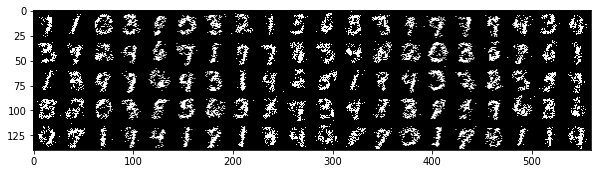
\includegraphics[height = 0.5\textwidth, width = 1\textwidth]{Exercise4/Report/rbm_ncomp_20_itr_20}
		\caption{n\_components = 20, n\_iterations = 20}\label{fig:rbm_ncomp_20_itr_20}
	\end{subfigure}%
	\begin{subfigure}[b]{0.33\textwidth}
		\centering
		\captionsetup{width=0.8\linewidth, format = hang}
		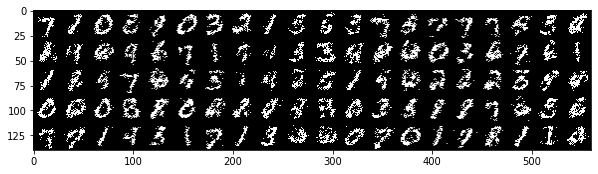
\includegraphics[height = 0.5\textwidth,width = 1\textwidth]{Exercise4/Report/rbm_ncomp_30_itr_30}
		\caption{n\_components = 30, n\_iterations = 30}\label{fig:rbm_ncomp_30_itr_30}
	\end{subfigure}
	\begin{subfigure}[b]{0.33\textwidth}
		\centering
		\captionsetup{width=0.8\linewidth, format = hang}
		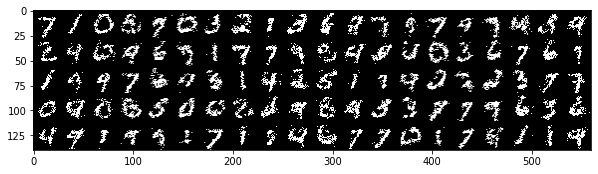
\includegraphics[height = 0.5\textwidth,width = 1\textwidth]{Exercise4/Report/rbm_ncomp_40_itr_40}
		\caption{n\_components = 40, n\_iterations = 40}\label{fig:rbm_ncomp_40_itr_40)}
	\end{subfigure}%
	\begin{subfigure}[b]{0.33\textwidth}
		\centering
		\captionsetup{width=0.8\linewidth, format = hang}
		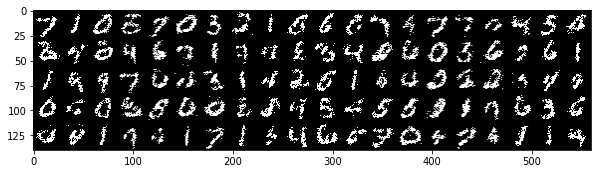
\includegraphics[height = 0.5\textwidth,width = 1\textwidth]{Exercise4/Report/rbm_ncomp_50_itr_50}
		\caption{n\_components = 50, n\_iterations = 50}\label{fig:rbm_ncomp_50_itr_50)}
	\end{subfigure}%
	\begin{subfigure}[b]{0.33\textwidth}
		\centering
		\captionsetup{width=0.8\linewidth, format = hang}
		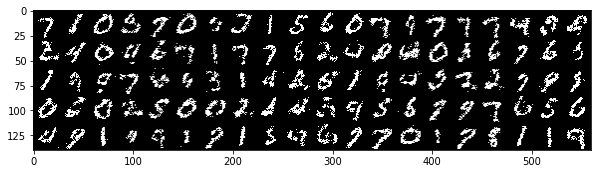
\includegraphics[height = 0.5\textwidth,width = 1\textwidth]{Exercise4/Report/rbm_ncomp_60_itr_60}
		\caption{n\_components = 60, n\_iterations = 60}\label{fig:rbm_ncomp_60_itr_60)}
	\end{subfigure}%
	\caption{Gibbs sampling on test images for different train parameter configurations}
	\label{fig:rbm_dig}
\end{figure}\\
From the model evaluation results on the test set it was observed that, change in any of these n\_components and n\_iterations parameters have the same impact on the model performance. Increasing these parameters increase the pseudo-likelihoods. For higher values of these parameters, the time taken for each iteration is higher. As seen from figure \ref{fig:rbm_dig}, the model performance for higher values of n\_components and n\_iterations is better compared to 20, 30 and 40. Except for the digits 2, 4 and 5, the model in figure \ref{fig:rbm_ncomp_60_itr_60)} does a good job in giving out better sampled images.  Now, to evaluate gibbs sampling steps, we fix the train parameters n\_components and n\_iterations to 40, learning rate to 0.01, batch size to 10 and vary the gibbs sampling steps. Few results are shown below.
\begin{figure}[ht]
	\begin{subfigure}[b]{0.33\textwidth}
		\centering
		\captionsetup{ width=1\linewidth, format = hang}
		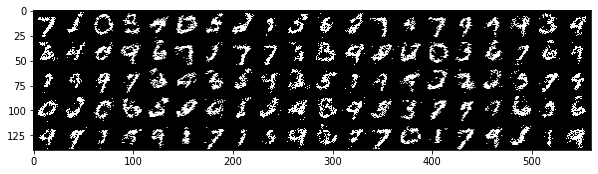
\includegraphics[height = 0.5\textwidth, width = 1\textwidth]{Exercise4/Report/rbm_gibbs_30}
		\caption{Gibbs sampling steps = 30}\label{fig:rbm_gibbs_30}
	\end{subfigure}%
	\begin{subfigure}[b]{0.33\textwidth}
		\centering
		\captionsetup{width=1\linewidth, format = hang}
		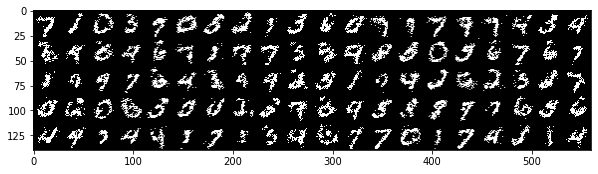
\includegraphics[height = 0.5\textwidth, width = 1\textwidth]{Exercise4/Report/rbm_gibbs_40}
		\caption{Gibbs sampling steps = 40}\label{fig:rbm_gibbs_40}
	\end{subfigure}%
	\begin{subfigure}[b]{0.33\textwidth}
		\centering
		\captionsetup{width=1\linewidth, format = hang}
		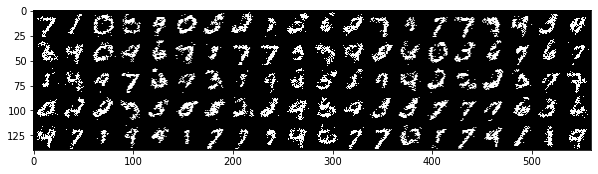
\includegraphics[height = 0.5\textwidth,width = 1\textwidth]{Exercise4/Report/rbm_gibbs_50}
		\caption{Gibbs sampling steps = 50}\label{fig:rbm_gibbs_50}
	\end{subfigure}
	\captionsetup{format = hang}
	\caption{Gibbs sampling on test images for different Gibbs sampling steps and constant train parameter configurations}
	\label{fig:rbm_gibbs_dig}
\end{figure}\\
From the figure \ref{fig:rbm_gibbs_dig} it can be seen that there is some improvement in the model performance for increase in gibbs sampling steps but not to a great extent.\\
\textbf{Reconstructing Missing parts :} 
\begin{table}[!htpb]
	\centering
	\begin{tabular}{|p{4cm}|p{2cm}|p{4cm}|p{4.5cm}|}
		\cellcolor{blue!25}Rows to be Removed & \cellcolor{blue!25} Gibbs Sampling Steps & \cellcolor{blue!25} Sampled Image with missing parts  & \cellcolor{blue!25} Reconstructed Image \\ \hline
		Top rows 1-10 & 30 & 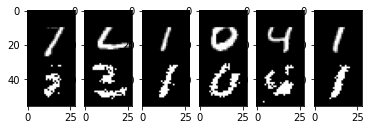
\includegraphics[height=1cm, width=3.5cm]{Exercise4/Report/reconst_gibs_30_row_1-10} & 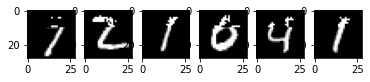
\includegraphics[height=1cm]{Exercise4/Report/reconst_gibs_30_row_1-10_1}\\ \hline
		Top rows 1-10 & 50 & 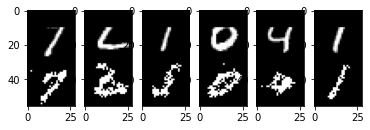
\includegraphics[height=1cm, width=3.5cm]{Exercise4/Report/reconst_gibs_50_row_1-10} & 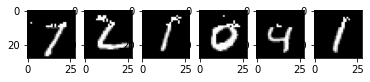
\includegraphics[height=1cm]{Exercise4/Report/reconst_gibs_50_row_1-10_1}\\ \hline
		Middle rows 10-20 & 30 & 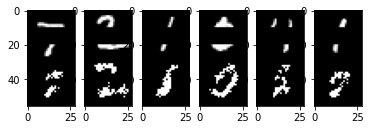
\includegraphics[height=1cm, width=3.5cm]{Exercise4/Report/reconst_gibs_30_row_10-20} & 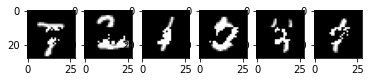
\includegraphics[height=1cm]{Exercise4/Report/reconst_gibs_30_row_10-20_1}\\ \hline
		Middle rows 10-20 & 50 & 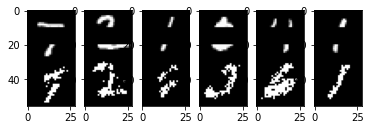
\includegraphics[height=1cm, width=3.5cm]{Exercise4/Report/reconst_gibs_50_row_10-20} & 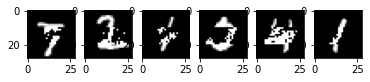
\includegraphics[height=1cm]{Exercise4/Report/reconst_gibs_50_row_10-20_1}\\ \hline
		End rows 17-27 & 30 & 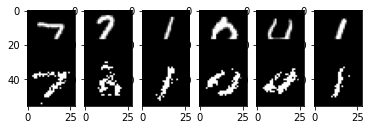
\includegraphics[height=1cm, width=3.5cm]{Exercise4/Report/reconst_gibs_30_row_17-27} & 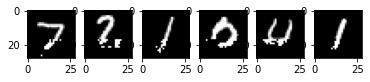
\includegraphics[height=1cm]{Exercise4/Report/reconst_gibs_30_row_17-27_1}\\ \hline
		End rows 17-27 & 50 & 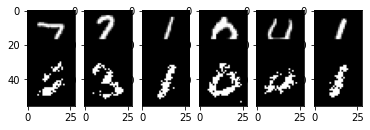
\includegraphics[height=1cm, width=3.5cm]{Exercise4/Report/reconst_gibs_50_row_17-27_1} & 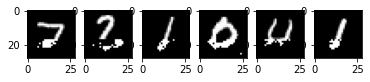
\includegraphics[height=1cm]{Exercise4/Report/reconst_gibs_50_row_17-27}\\ \hline
		\end{tabular}
	\captionsetup{format = hang}
	\caption{RBM performance for reconstructing missing parts of image with model parameters as n\_components=50, n\_iterations=50, learning rate = 0.01, batch size = 10}
	\label{table:4.1}
\end{table}
It is observed that, increasing the number of components, number of epochs  and gibbs sampling steps the model makes reconstruct better. Reducing or increasing the learning rate has poor performance on the model output. The table \ref{table:4.1} summarizes the results of a RBM in reconstructing the images. It can be seen that the model gives better results when top rows are removed compared to middle and end rows.
\section{Deep Boltzmann Machines}
Deep Boltzmann Machines (DBM's) are nothing but RBM's stacked on one another. The features extracted from one layer of DBM is passed to the second layer of DBM. By doing this the model learns the image features in a better way. The figure shows the features of RBM with 50 components (hidden units) from the above exercise and the feature of 2 layers of DBM. 
\begin{figure}[ht]
	\begin{subfigure}[b]{0.33\textwidth}
		\centering
		\captionsetup{ width=0.9\linewidth, format = hang}
		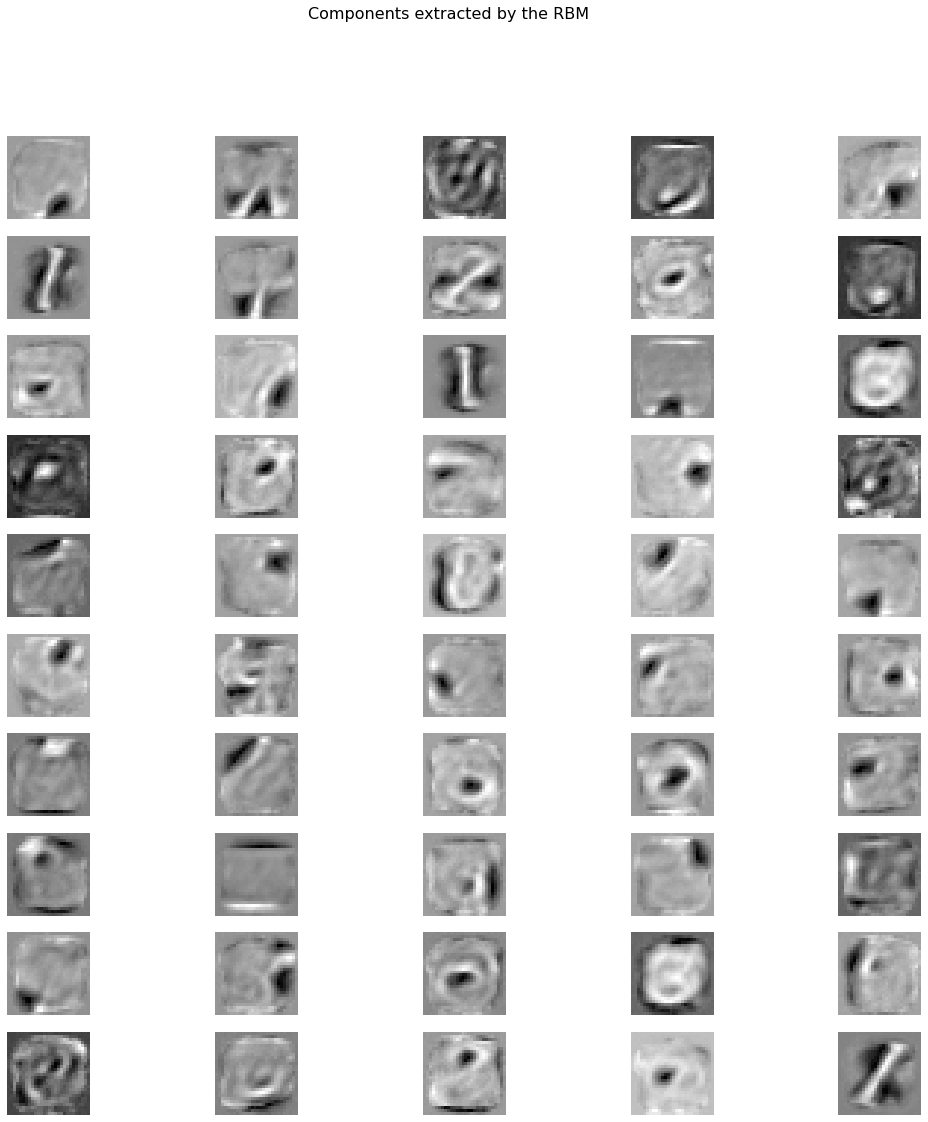
\includegraphics[height = 0.8\textwidth, width = 0.95\textwidth]{Exercise4/Report/rbm_features}
		\caption{Feature map of RBM from previous section}\label{fig:rbm_features}
	\end{subfigure}%
	\begin{subfigure}[b]{0.33\textwidth}
		\centering
		\captionsetup{width=0.9\linewidth, format = hang}
		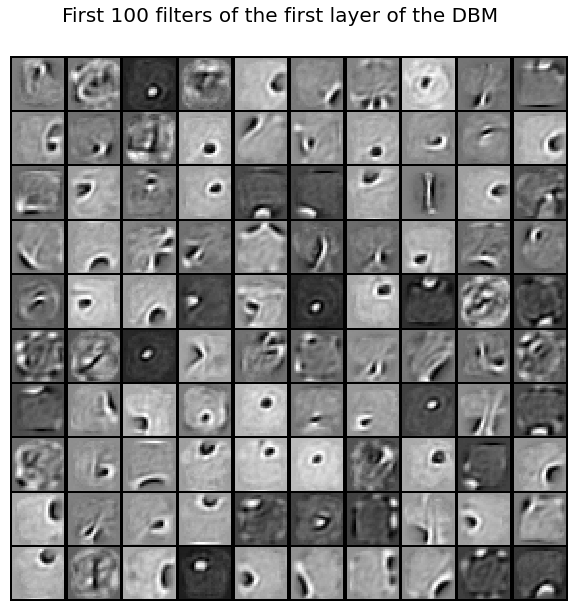
\includegraphics[height = 0.8\textwidth, width = 0.95\textwidth]{Exercise4/Report/dbm_feature_1}
		\caption{Feature Map of 1st layer of DBM}\label{fig:dbm_features_1}
	\end{subfigure}%
	\begin{subfigure}[b]{0.33\textwidth}
		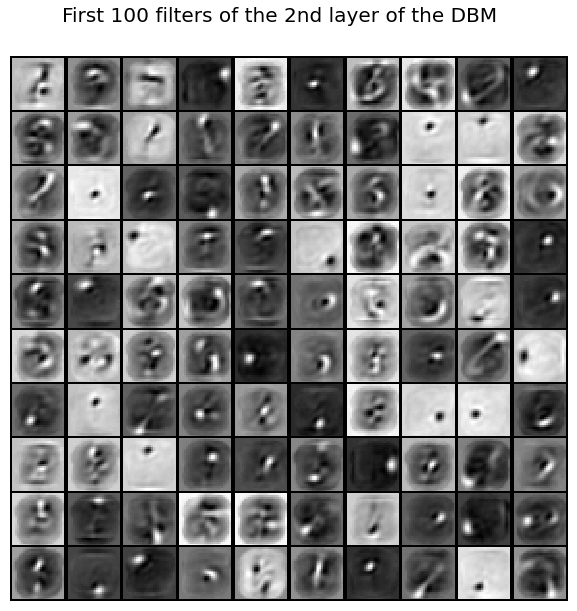
\includegraphics[height = 0.8\textwidth,width = 0.95\textwidth]{Exercise4/Report/dbm_feature_2}
		\caption{Feature Map of 2nd layer of DBM}\label{fig:dbm_features_2}
		\centering
		\captionsetup{width=0.9\linewidth, format = hang}
	\end{subfigure}
	\captionsetup{format = hang}
	\caption{Features maps of DBM and RBM}
	\label{fig:features}
\end{figure}
\begin{wrapfigure}{L}{0.38\textwidth}
	\vspace*{-0.9cm}
	\captionsetup{format = hang}
	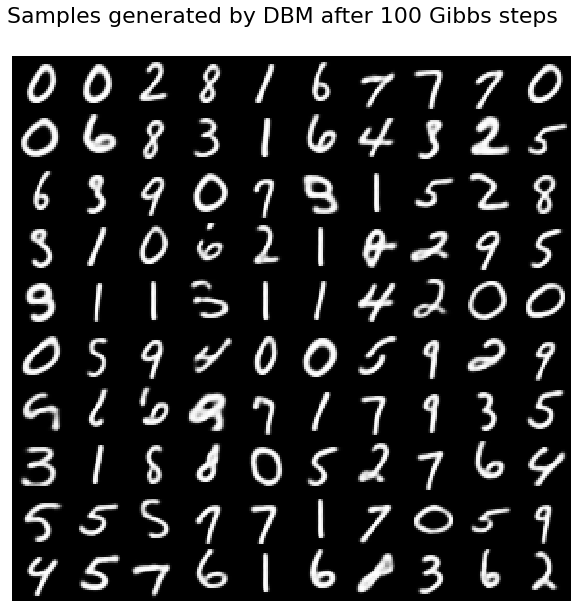
\includegraphics[height = 0.8\textwidth,width = 1\textwidth]{Exercise4/Report/dbm_output}
	\caption{DBM samples after 100 Gibbs steps}\label{fig:dbm}
\end{wrapfigure}%

The figure \ref{fig:dbm_features_1} shows layer 1 basic features of DBM which are extracted from the layer 1 filters. Figure 2 shows the layer 2 edge features of DBM. It is evident that the feature maps of DBM is better than RBM as DBM has more filters as compared with RBM with 50 components as shown in figure \ref{fig:rbm_features}. The deeper the network, the better the extracted input features are and so is the model's performance. Since the DBM model has better feature maps with 2 layers and more number of hidden units than a RBM model, the result of DBM shown in figure \ref{fig:dbm} is more clear and accurate than a RBM model.\\
\section{Generative Adversarial Networks}
As in their name, GAN's can generate new synthetic data using two different neural networks namely the generator and the discriminator. The generator generates a new instance while the discriminator tries to distinguish the generated data from the ones in the training set and assigns a probability to every new data generation that if a sample corresponds to any from training set or a fake. This way both the neural networks compete in a zero-sum game trying to maximize their performance.  In this exercise, we analyze the GAN's using Cifar dataset. We train the GAN's for 15000 batches and notice that the model generates car images with  D-loss : 0.6914 D-acc : 0.5136 G-loss : 0.6746 and G-acc : 0.3147. The generated images seems to be of poor resolution and they are kind of blurry. May be this output could be improved by increasing the batch size as well as number of epochs. Some of the generated images for batches 10000 and 15000 are given in the below figure 
\begin{figure}[ht]
	\begin{subfigure}[b]{0.4\textwidth}
		\centering
		\captionsetup{ width=0.9\linewidth, format = hang}
		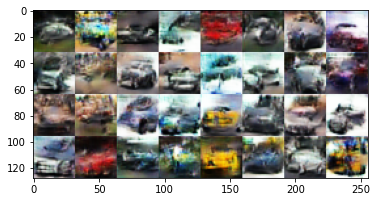
\includegraphics[height = 0.8\textwidth, width = 0.95\textwidth]{Exercise4/Report/gans_1}
		\caption{After 10000 batches}\label{fig:gan_1}
	\end{subfigure}%
	\begin{subfigure}[b]{0.4\textwidth}
		\centering
		\captionsetup{width=0.9\linewidth, format = hang}
		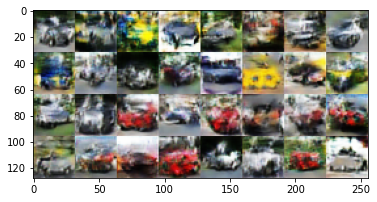
\includegraphics[height = 0.8\textwidth, width = 0.95\textwidth]{Exercise4/Report/gans_2}
		\caption{After 15000 batches}\label{fig:gan_2}
	\end{subfigure}%
	\captionsetup{format = hang}
	\caption{GAN image generation}
	\label{fig:gan}
\end{figure}
\section{Optimal transport}
This exercise deals with color transport between two images where the color palette of one image is imposed on the other. This means, after the color transport the color distribution of the resultant image will be very close to the input image. For this purpose we use two distance metrics namely Wasserstein metrics and Sinkhorn  metrics. The transport of the color distribution is done using these distance which is a measure of work done i.e., to transport the mass of one distribution to another.  Figure \ref{fig:ot_scatterplot} shows the color distribution scatters of the two images. Figure \ref{fig:ot_out} shows the resultants of these color transports. The first column of images in figure \ref{fig:ot_out} are the input images. The second column shows the optimal transport using  Wasserstein distance and the third column corresponds to Sinkhorn distances. It can be seen from these images that using Wasserstein distance makes the output images very sharp but they can preserve minute details of the original images. On the other hand Sinkhorn distance does a better job by giving a smooth and clear output due to the fact that it uses entropy to regularize the two distributions.
\newpage
\begin{figure}[!htpb]
	\begin{subfigure}[b]{0.45\textwidth}
		\centering
		\captionsetup{format = hang}
		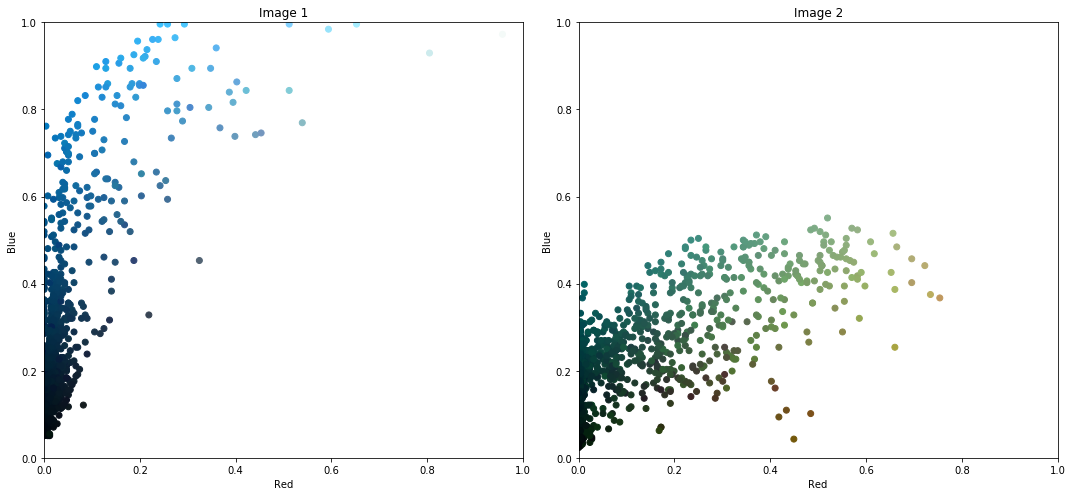
\includegraphics[height = 0.5\textwidth,width = 1\textwidth]{Exercise4/Report/ot_scatterplot}
		\caption{Color scatters of image 1 and image 2  }\label{fig:ot_scatterplot}
	\end{subfigure}%
	\begin{subfigure}[b]{0.45\textwidth}
		\centering
		\captionsetup{width=0.9\linewidth, format = hang}
		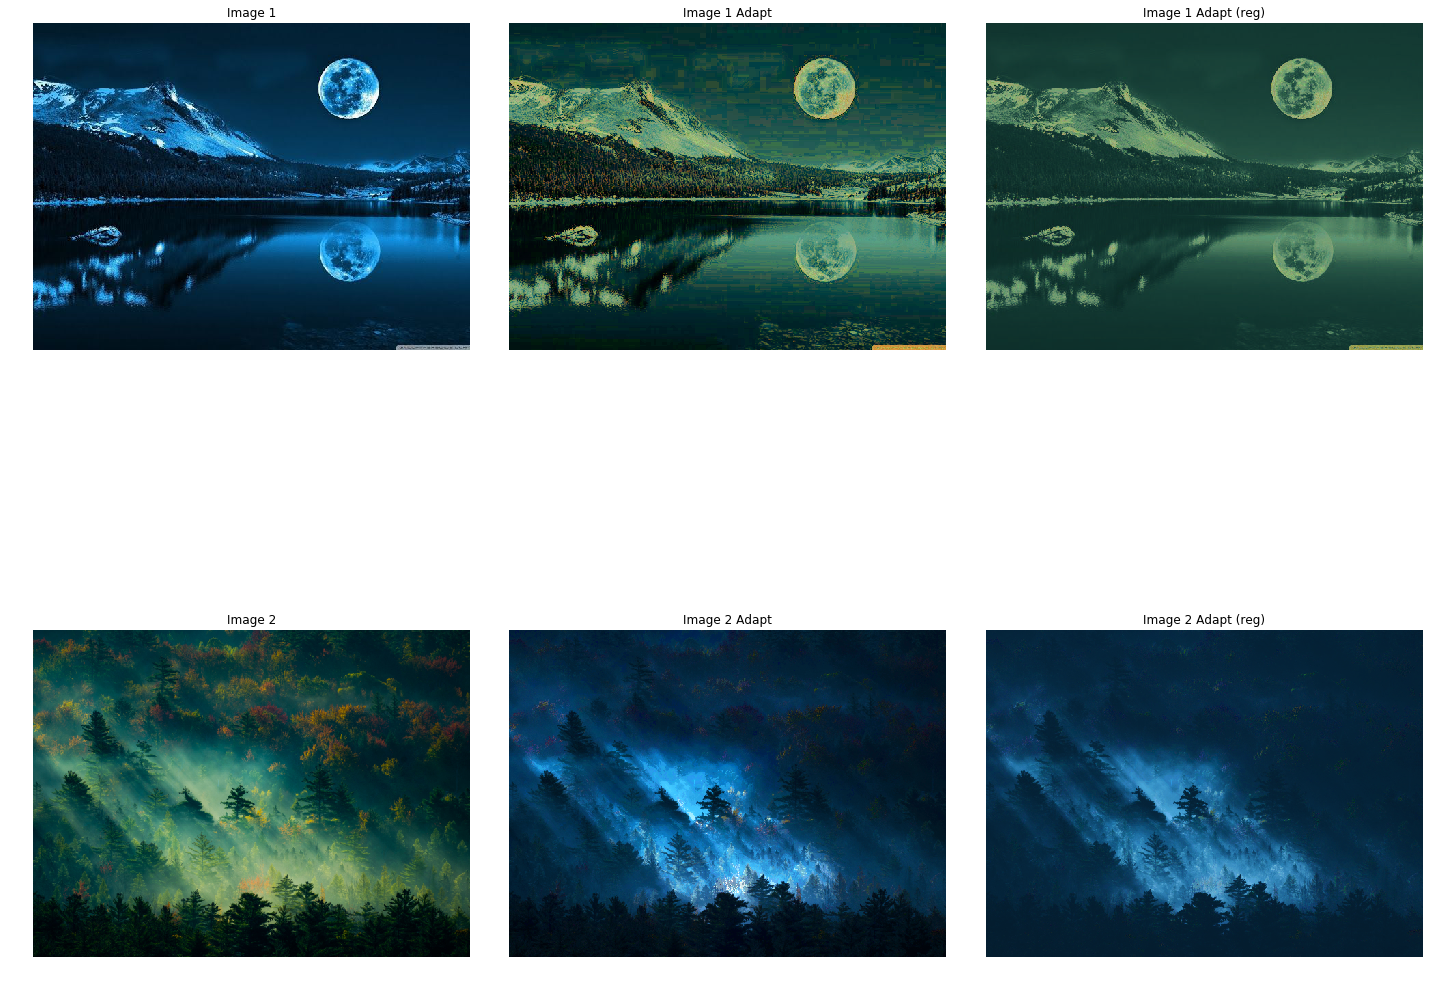
\includegraphics[height = 0.8\textwidth, width = 1\textwidth]{Exercise4/Report/ot_output}
		\caption{Color Swapped Images}\label{fig:ot_out}
	\end{subfigure}%
	\captionsetup{format = hang}
	\caption{Optimal color transport between two images}
	\label{fig:ot}
\end{figure}
We then compare a standard GAN with Wasserstein GAN by training and evaluating them on MNIST dataset. We train each of the models with the following parameter configuration; batches = 20000 , batch size=64 and plot interval = 500. The results of these GAN's are shown in the table \ref{table:4.2} for 1000, 10000 and 20000 batches of training. It was observed that, a standard GAN takes lesser time in training around 65 iteration per seconds. At the end of 20000 iterations we get  the loss and accuracies of the discriminator and generator as D-loss: 0.5373 D-acc: 0.7344 G-loss: 1.3259 G-acc: 0.125. The generated images are not of high quality and accuracy. They also contain salt and pepper noise as seen for 1st row of table \ref{table:4.2}. These GAN's suffer from weight clipping where all the weights of the GAN's vary only between a range $[min,max]$ values. Due to this they cannot model complex structures as their learning is restricted. To overcome this issue Wasserstein GAN's.

In Wasserstein GAN with weight clipping, the GAN uses a clipping that restricts the maximum weight value in its function. This means, the learning is controlled by the clipping hyper parameter. With this the model performance improves a bit as seen from row 2 of table \ref{table:4.2}. The performance of this WGAN with clipping depends on the tuning of the clipping parameter. A smaller value of this could cause vanishing gradients and larger value could cause longer time for the weights to reach their limits. Therefore, we move on to Wasserstein GAN with gradient penalty.

The issues of weight clipping is solved by using a weight penalty that enforces the gradients to have a norm 1 if they move away from their target norm. This method produces some good quality images as seen from row 3 of table \ref{table:4.2}. Training this model takes more time of around 13 iterations per seconds compared to other two models. 


\begin{table}[!htpb]
	\centering
	\begin{tabular}[t]{|>{\centering}p{2cm}|p{4.6cm}|p{4.6cm}|p{4.6cm}|}

		\cellcolor{blue!25}GAN Techniques & \cellcolor{blue!25} GAN output at batch 1000 & \cellcolor{blue!25} GAN output at batch 10000   & \cellcolor{blue!25} GAN output at batch 20000 \\ \hline
		Standard GAN & 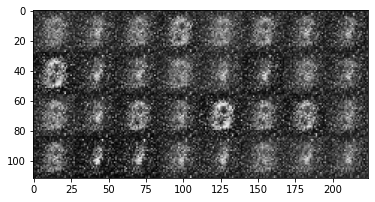
\includegraphics[height=3cm, width=4.4cm]{Exercise4/Report/GAN_999} &  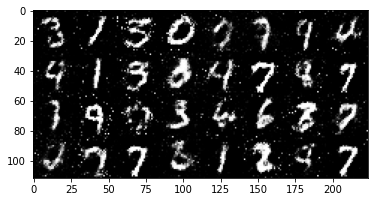
\includegraphics[height=3cm, width=4.4cm]{Exercise4/Report/GAN_9999} & 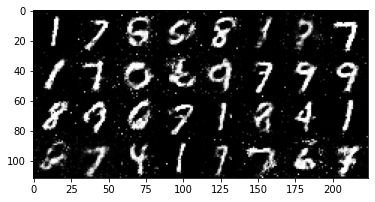
\includegraphics[height=3cm, width=4.4cm]{Exercise4/Report/GAN_20000}\\ \hline
		
		Wasserstein GAN with Weight Clipping & 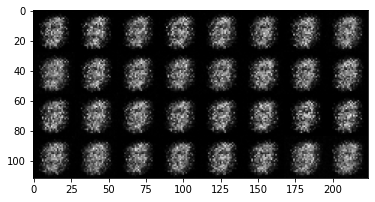
\includegraphics[height=3cm, width=4.4cm]{Exercise4/Report/WGAN_WC_999} &  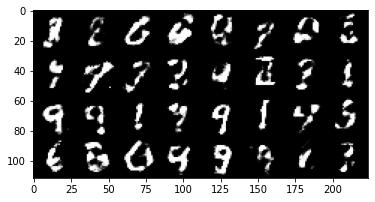
\includegraphics[height=3cm, width=4.4cm]{Exercise4/Report/WGAN_WC_9999} & 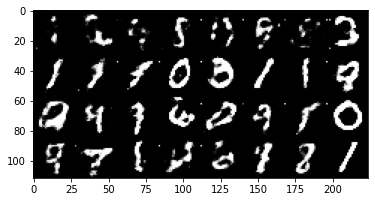
\includegraphics[height=3cm, width=4.4cm]{Exercise4/Report/WGAN_WC_20000}\\ \hline
			
		
		Wasserstein GAN with Gradient Penalty & 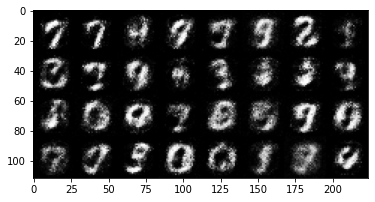
\includegraphics[height=3cm, width=4.4cm]{Exercise4/Report/WGAN_GP_499} &  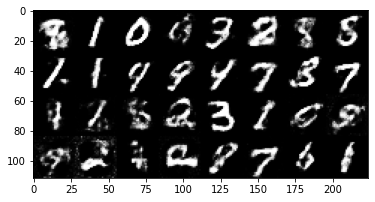
\includegraphics[height=3cm, width=4.4cm]{Exercise4/Report/WGAN_GP_9999} & 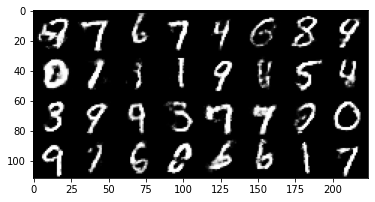
\includegraphics[height=3cm, width=4.4cm]{Exercise4/Report/WGAN_GP_20000}\\ \hline	

	\end{tabular}
	
	\captionsetup{format = hang}
	\caption{Results of standard GAN and WGAN's trained on MNIST dataset}
	\label{table:4.2}
\end{table}